\clearpage{\pagestyle{empty}\cleardoublepage}

\chapter{Risultati ottenuti}

\begin{flushright}\begin{small}\textit{"Hard science gives sensational results\\ with a horribly boring process."}\\
- Nassim Nicholas Taleb -\\
\end{small}\end{flushright}

Lo sviluppo e la convalida dell'algoritmo sono stati permessi dall'applicazione di quest'ultimo ad apposite immagini in fluorescenza rossa di sferette di calibrazione e di cellule di fibroblasti.

Le immagini di riferimento, utilizzate nella prima e nella seconda fase del programma, sono state acquisite in otto pozzetti di una multiwell: due con sferette ad intensità relativa del 100\% e due del 10\%, una con una mixture di cinque intensità (1\%, 3\%, 10\%, 30\% e 100\%) ed una con quattro intensità, infine nelle rimanenti è stato posto unicamente il mezzo di coltura, così da studiare la fluorescenza di background indotta dalla sorgente.
Il riempimento di ogni pozzetto ha previsto l'agitazione sia manuale che con sonificatore delle sferette e l'iniezione con le pipette ghilson di $220\ \mu l$ di terreno completo e di sferette di calibrazione: $10\ \mu l$ per i quattro pozzetti ad intensità unica, $2\ \mu l$ e $2.5\ \mu l$ rispettivamente per quello con cinque e quattro intensità.

L'analisi che segue mostra grafici e risultati dell'algoritmo applicato all'immagine dei fibroblasti, corretta tramite una prima immagine di calibrazione costituita da un campione di sferette con intensità relativa del 10\% ed una seconda contenente cinque intensità differenti. 
L'attenzione viene posta in particolare sull'efficacia dell'algoritmo nella rimozione dell'``effetto dei bordi'', poiché come visto in precedenza il difetto della fluorescenza di sfondo viene semplicemente eliminato sottraendo il parametro costante identificato nella seconda fase.

I buoni risultati conseguiti dall'algoritmo possono essere percepiti dall'osservazione degli istogrammi delle distribuzioni di intensità, dal cambiamento sostanziale del p-value associato alla dipendenza spaziale della luminescenza rilevata ed infine dall'analisi qualitativa dell'evoluzione delle immagini nelle varie fasi dell'elaborazione.

Osserviamo inoltre che prima di giungere ai risultati finali di seguito riportati l'algoritmo è stato via via migliorato: ad esempio, si è constatato che la curva in grado di fittare al meglio i centri di sferette nella prima fase dell'algoritmo fosse, anziché una polinomiale, una curva di tipo esponenziale, che l'intensità da associare ad ogni punto di massimo fosse meglio interpretarla come intensità integrale media piuttosto che puntuale ed inoltre sono stati ricavati ed inseriti i valori ottimali dei parametri utilizzati nei vari passaggi di elaborazione dell'immagine.

\section{Distribuzione delle intensità}

Come visto, l'``effetto dei bordi'' consiste nel fatto che il microscopio crei immagini con intensità maggiore al centro rispetto al margine, comportando di conseguenza un'alterazione della distribuzione delle intensità. 
Tale fenomeno viene attenuato in modo sostanziale tramite l'azione della prima fase dell'algoritmo, la quale agisce proprio sul difetto preso in considerazione.

Il cambiamento della distribuzione di intensità provocato dal software è percepibile graficando gli istogrammi relativi alle varie intensità rilevate all'interno dell'immagine in fase pre e post correzione.

Il miglioramento più evidente da questo punto di vista si ha nell'istogramma della prima immagine di calibrazione (\figurename~\ref{fig:isto1}), poiché le intensità, prima distribuite entro un range molto ampio, risultano molto più piccate attorno un unico valore.
Tale risultato è proprio ciò a cui si mirava, dato che le sferette contenute nel campione risultano avere la medesima intensità.

Anche in \figurename~\ref{fig:isto2} si nota un netto miglioramento, infatti le cinque gaussiane associate ai differenti valori di intensità relativa delle sferette mostrano a posteriori dell'elaborazione un'apertura, ossia una covarianza, molto minore ed una miglior definizione dei confini tra l'una e l'altra. 

D'altra parte, gli istogrammi associati all'immagine volta a correzione, ovvero quella delle cellule, non presentano sostanziali cambiamenti, a meno di una migliore simmetria della distribuzione delle intensità presenti nell'immagine.
Tale risultato era in realtà prevedibile, dato che in tal caso non si tratta più di un'immagine di calibrazione, quindi creata per poter mostrare determinate proprietà luminescenti, bensì di un'immagine reale e di natura biologica. 
Per tale motivo le intensità rilevate nell'immagine è giusto che si estendano entro un range abbastanza ampio, proprio perché a seconda della concentrazione delle probes fluorescenti nella cellula sarà differente il grado di luminosità sviluppato.

\begin{figure}
 \centering
 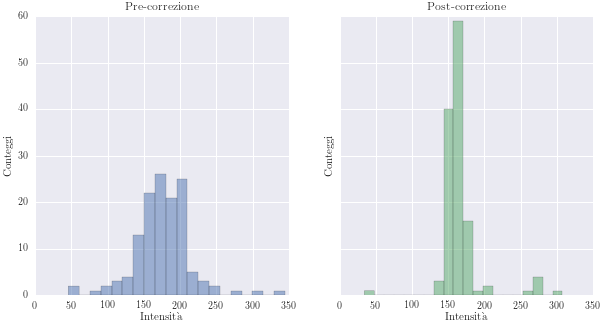
\includegraphics[scale=.42]{img/CAP4isto1.png}
 \caption{\small{Istogrammi pre e post correzione relativi alla prima immagine di calibrazione. Sulle ordinate è riportato il numero di occorrenze, sulle ascisse l'intensità.}}
 \label{fig:isto1}
\end{figure}

\begin{figure}
 \centering
 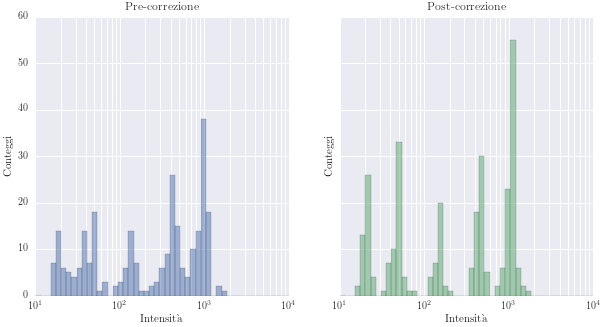
\includegraphics[scale=.42]{img/CAP4isto2.png}
 \caption{\small{Istogrammi pre e post correzione, in scala logaritmica, relativi alla seconda immagine di calibrazione. Sulle ordinate è riportato il numero di occorrenze, sulle ascisse l'intensità.}}
 \label{fig:isto2}
\end{figure}

\begin{figure}
 \centering
 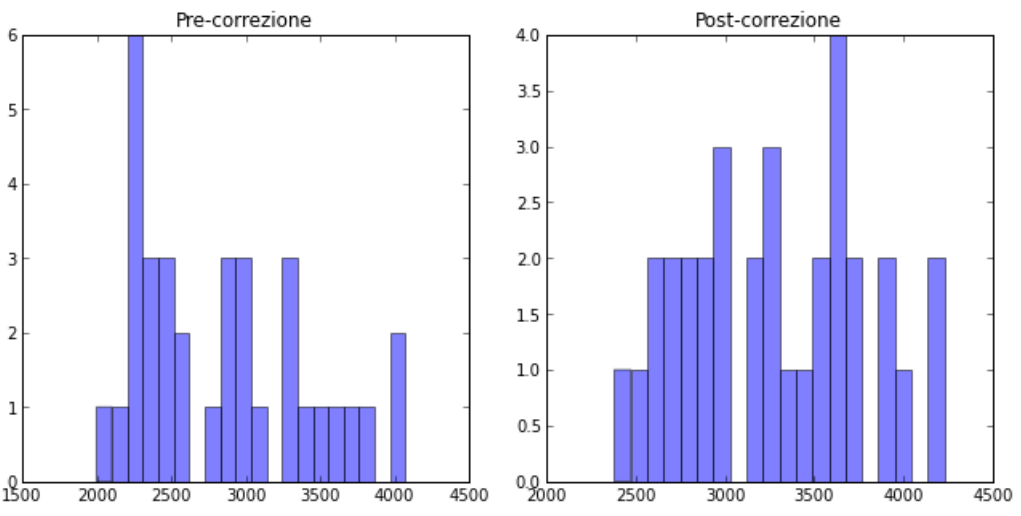
\includegraphics[scale=.42]{img/CAP4isto3.png}
 \caption{\small{Istogrammi pre e post correzione relativi all'immagine delle cellule. Sulle ordinate è riportato il numero di occorrenze, sulle ascisse l'intensità.}}
 \label{fig:isto3}
\end{figure}


\section{Dipendenza spaziale dell'intensità}

In statistica, data un'ipotesi nulla ($H_0$), questa la si può accettare o rifiutare sulla base del cosiddetto \textit{p-value}, parametro probabilistico con valore compreso tra 0 ed 1.
Esso può essere definito come livello di significatività assegnato e quantifica la ``forza dell'evidenza'' contro l'ipotesi nulla $H_0$, a favore dell'alternativa, espressa dai dati osservati su un determinato campione. 
Per esempio, assegnato un valore di soglia, se il p-value è maggiore di tale valore allora $H_0$ non viene rigettata, in caso contrario sì.
Di conseguenza il p-value esprime quanto sia plausibile che i dati osservati si ottengano essendo vera l’ipotesi nulla: un p-value grande esprime evidenza sperimentale a favore dell'ipotesi nulla, mentre un suo valore piccolo un'evidenza a favore dell'ipotesi alternativa.

Come precedentemente osservato, l'``effetto dei bordi'' comporta l'instaurarsi di una dipendenza dell'intensità del pixel dalla posizione di quest'ultimo: è proprio la ``forza'' di questa relazione funzionale che può essere misurata tramite il valore del p-value.
A tal proposito è stata valutata per ogni punto di massimo dell'immagine (centro delle sferette per le immagini di calibrazione e nuclei delle cellule per l'immagine da correggere) la distanza dall'origine, intesa come punto centrale dell'immagine stessa, così da ottenere un set di dati costituito da una sorta di distanze radiali. 
Per ottenere il valore del p-value si è quindi sfruttata la funzione \textit{linregress}, in grado di valutare la relazione lineare esistente o meno tra le intensità dei punti di massimo e le distanze radiali associate.
Tale funzione restituisce il p-value come semplice parametro di return e questo viene valutato prendendo come ipotesi nulla $H_0$ il fatto che la slope sia nulla, quindi maggiore sarà il p-value maggiore e più corretto sarà assumere l'assenza di una dipendenza spaziale dell'intensità.

\begin{figure}
 \centering
 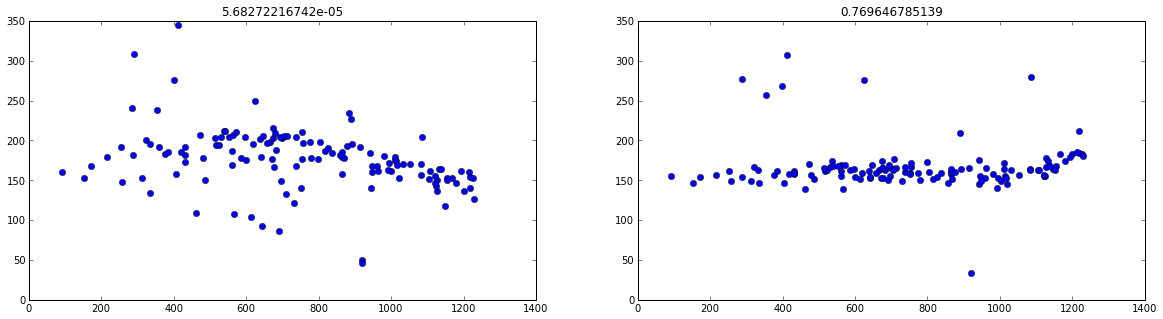
\includegraphics[scale=.50]{img/CAP4pvalue1.png}
 \caption{\small{Distribuzione delle intensità in funzione della distanza radiale per la prima immagine di calibrazione. Il grafico in alto è relativo alla fase di pre-correzione ed in basso alla fase di post-correzione. I valori riportati al di sopra sono i p-value corrispondenti alle rispettive regressioni lineari.}}
 \label{fig:pvalue1}
\end{figure}

\begin{figure}
 \centering
 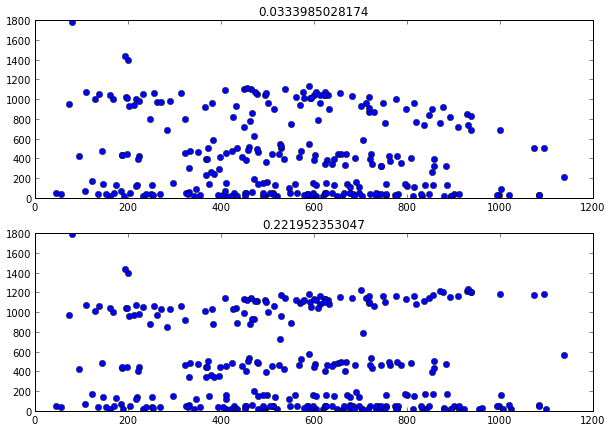
\includegraphics[scale=.50]{img/CAP4pvalue2.png}
 \caption{\small{Distribuzione delle intensità in funzione della distanza radiale per la seconda immagine di calibrazione. Il grafico in alto è relativo alla fase di pre-correzione ed in basso alla fase di post-correzione. I valori riportati al di sopra sono i p-value corrispondenti alle rispettive regressioni lineari.}}
 \label{fig:pvalue2}
\end{figure}

\begin{figure}
 \centering
 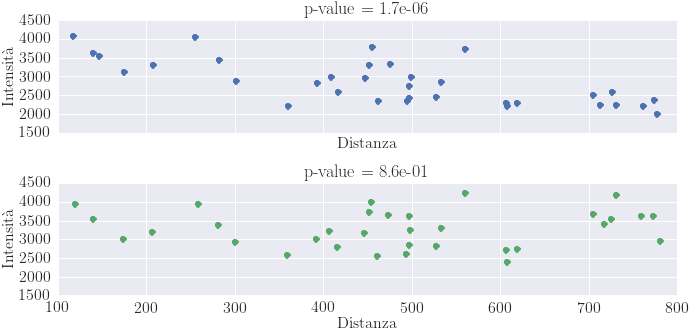
\includegraphics[scale=.50]{img/CAP4pvalue3.png}
 \caption{\small{Distribuzione delle intensità in funzione della distanza radiale per l'immagine delle cellule di fibroblasti. Il grafico in alto è relativo alla fase di pre-correzione ed in basso alla fase di post-correzione. I valori riportati al di sopra sono i p-value corrispondenti alle rispettive regressioni lineari.}}
 \label{fig:pvalue3}
\end{figure}

Come si evince dalle Figure \ref{fig:pvalue1}, \ref{fig:pvalue2}, \ref{fig:pvalue3}, il p-value viene altamente modificato dall'algoritmo e fatto crescere verso valori sempre più prossimi ad uno, comportando quindi una notevole diminuzione della correlazione esistente tra intensità e distanza radiale, sia nelle immagini di calibrazione che nell'immagine dei fibroblasti. 
Sulla base di tale analisi, dopo aver corretto l'immagine la dipendenza spaziale dell'intensità, inizialmente presente a causa della disomogeneità dell'illuminazione creata dalla sorgente, può essere considerata sostanzialmente non significativa.


\section{Analisi qualitativa}

Anche dalla semplice osservazione delle immagini è possibile notare i cambiamenti apportati dall'algoritmo.

In \figurename~\ref{fig:lg1} è possibile notare la sostanziale correzione del difetto della luminosità disomogenea: le sferette aventi stessa intensità, originariamente percepite con differente luminosità, vengono rappresentate dopo la correzione con una medesima tonalità di colore, mostrando così la realtà del campione.

\begin{figure}
 \centering
 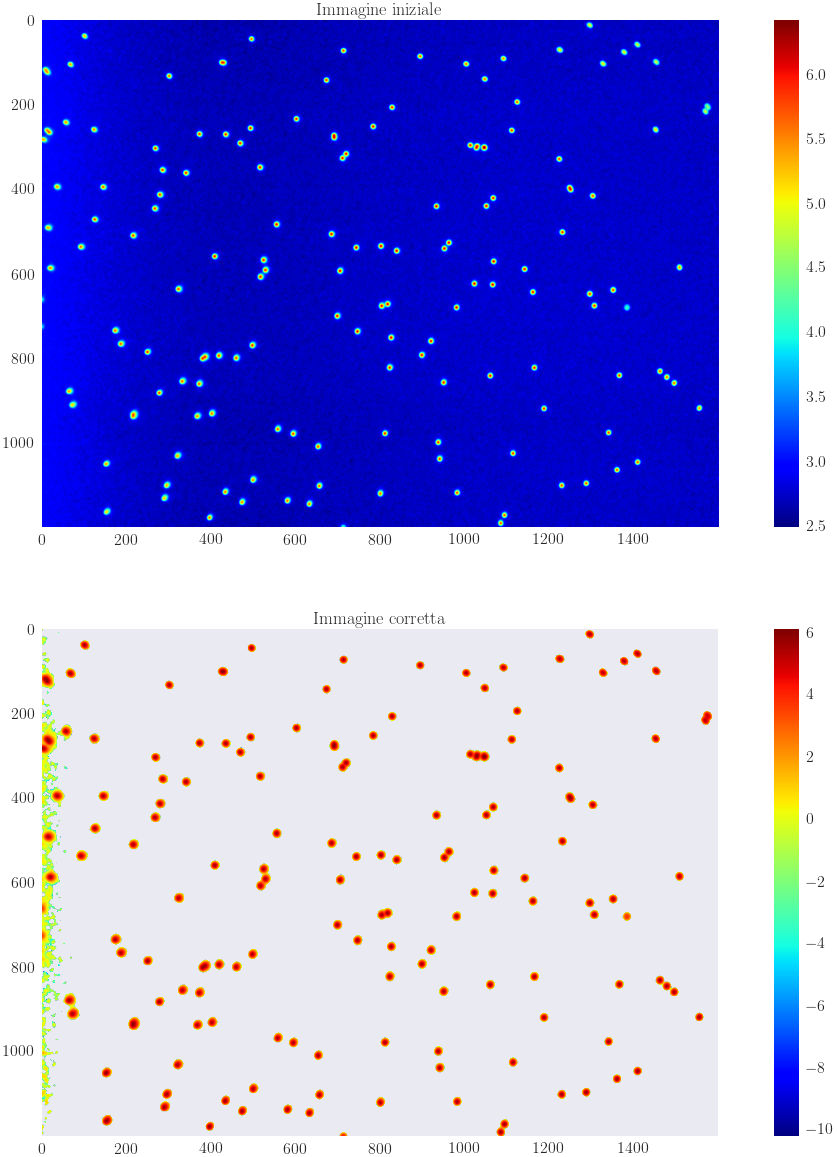
\includegraphics[scale=.40]{img/CAP4lg1.png}
 \caption{\small{Evoluzione della prima immagine di calibrazione: in alto è raffigurata quella acquisita del microscopio a fluorescenza e in basso quella risultante dopo aver corretto l'``effetto dei bordi''. Per un'interpretazione più intuitiva le immagini raffigurate sono i logaritmi delle corrispettive immagini originali, a cui è stato applicato ulteriormente il filtro gaussiano.}}
 \label{fig:lg1}
\end{figure}

Nell'evoluzione dell'immagine di calibrazione delle sferette aventi cinque intensità differenti (\figurename~\ref{fig:lg2}) è possibile notare, oltre alla correzione della disomogeneità spaziale delle intensità, anche la rimozione della fluorescenza residua di sfondo.

\begin{figure}
 \centering
 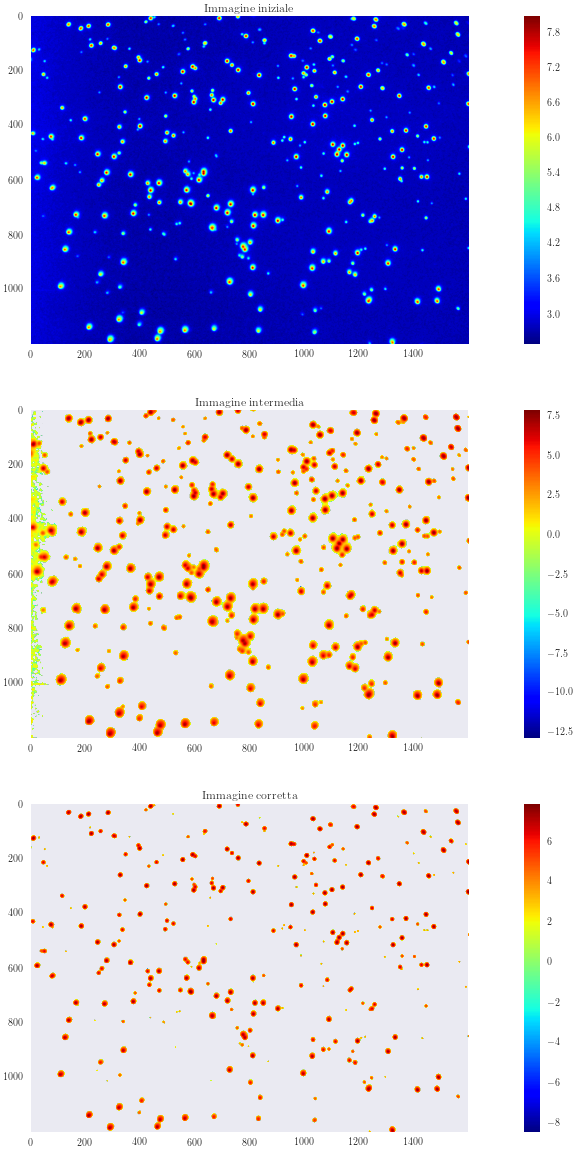
\includegraphics[scale=.50]{img/CAP4lg2.png}
 \caption{\small{Evoluzione della seconda immagine di calibrazione: in alto è raffigurata quella acquisita del microscopio a fluorescenza, al centro quella risultante dopo aver corretto l'``effetto dei bordi'' e in basso l'immagine privata del parametro costante di background. Per un'interpretazione più intuitiva le immagini raffigurate sono i logaritmi delle corrispettive immagini originali, a cui è stato applicato ulteriormente il filtro gaussiano.}}
 \label{fig:lg2}
\end{figure}

Per quanto riguarda l'immagine delle cellule di fibroblasti, vero target dell'algoritmo di correzione, il cambiamento risulta davvero ben evidente: il difetto dei bordi è fortemente attenuato, infatti i nuclei più a margine riacquistano una colorazione molto più intensa e confrontabile con quella dei nuclei centrali, ed il background viene pressochè portato a zero, il tutto pur mantenendo ben definiti i confini delle varie cellule.
Le varie fasi correttive dell'immagini sono ben evidenti sia in (\figurename~\ref{fig:lg3}) che in (\figurename~\ref{fig:cmap}).

\begin{figure}
 \centering
 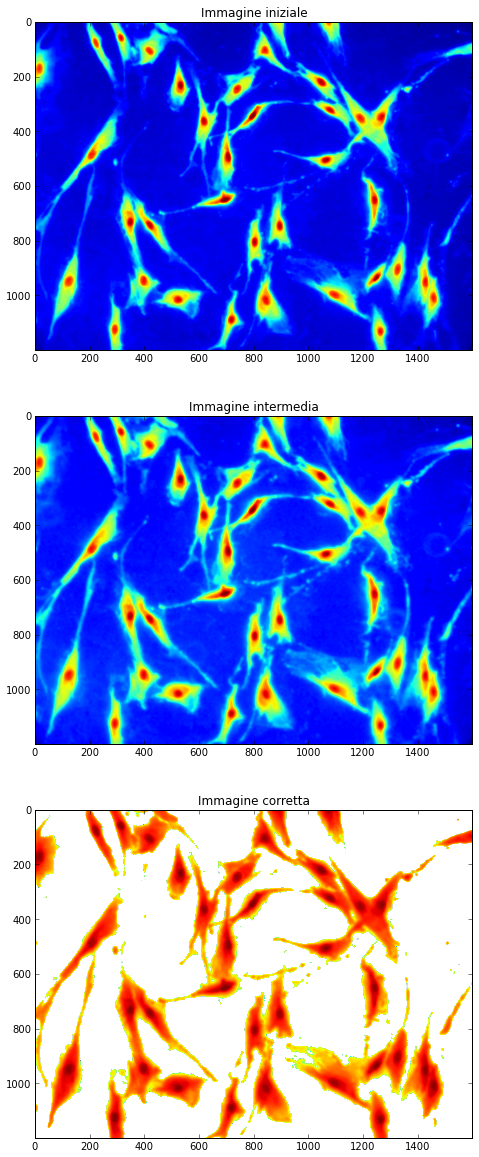
\includegraphics[scale=.50]{img/CAP4lg3.png}
 \caption{\small{Evoluzione della seconda immagine di calibrazione: in alto è raffigurata quella acquisita del microscopio a fluorescenza, al centro quella risultante dopo aver corretto l'``effetto dei bordi'' e in basso l'immagine privata del parametro costante di background. Per un'interpretazione più intuitiva le immagini raffigurate sono i logaritmi delle corrispettive immagini originali, a cui è stato applicato ulteriormente il filtro gaussiano.}}
 \label{fig:lg3}
\end{figure}

\begin{figure}
 \centering
 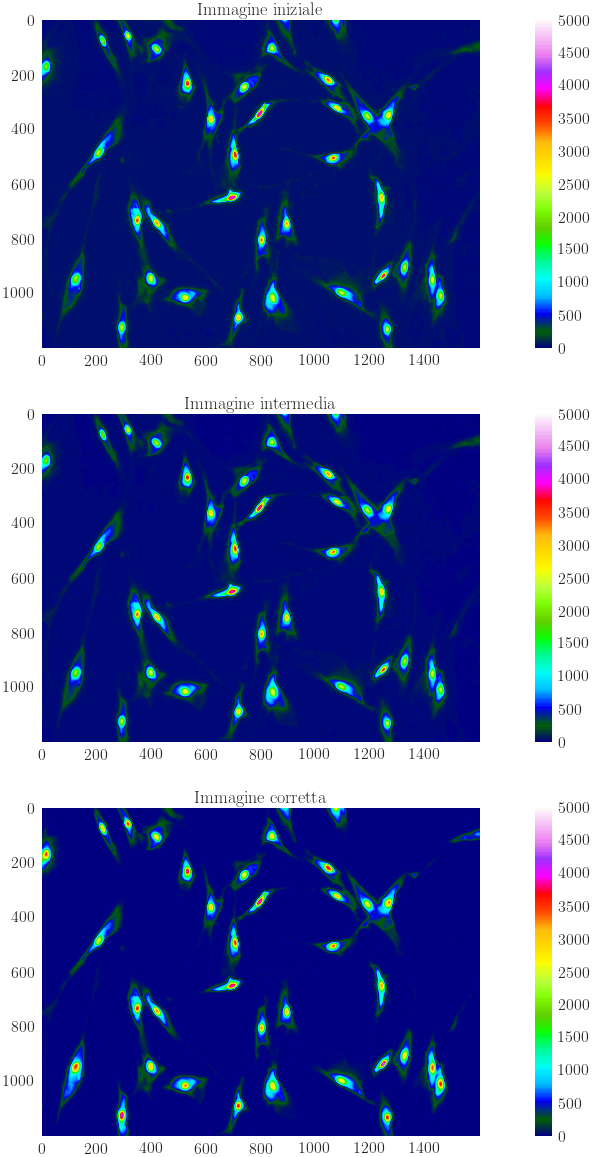
\includegraphics[scale=.50]{img/CAP4cmap.png}
 \caption{\small{Evoluzione della seconda immagine di calibrazione: in alto è raffigurata quella acquisita del microscopio a fluorescenza, al centro quella a cui sono stati sottratti i parametri costanti di background ed in basso l'immagine risultante dopo aver corretto l'ulteriore difetto della disomogeneità dell'illuminazione. Per un'interpretazione più intuitiva le immagini raffigurate sono le corrispettive immagini originali a cui è stato applicato il filtro gaussiano, rappresentate nella colour map ``gist\_ncar'', riportata a fianco.}}
 \label{fig:cmap}
\end{figure}